\documentclass[11pt]{article}

\usepackage{common}
\usepackage{amsmath}
\DeclareMathOperator*{\E}{\mathbb{E}}
\DeclareMathOperator*{\R}{\mathbb{R}}
\usepackage{booktabs}

\title{HW2: Language Modeling}
\author{Emily Tseng \\ et397@cornell.edu}
\begin{document}

\maketitle{}
\section{Introduction}

In a sense, a language is just a set of community-driven rules for what words should appear in what order. Language modeling is a generative problem that attempts to formalize this ordering by computing a probability distribution over a given sequence. As an example, consider the incomplete sentence ``\textit{Tickets were sold out for the 2 p.m. \_\_\_\_\_}'' A language model properly trained over the English language would compute a greater probability for the next word being ``\textit{movie}'' than, say, ``\textit{banana}''. 

The task is to generate a distribution as close as possible to the true distribution of your source language; or, in empirical terms, to maximize the probability (or minimize the perplexity) of your test set being drawn from your estimated distribution. In this homework, we use data from the Penn Treebank \citep{marcus-etal-1993-building} to implement and assess the following:

\begin{enumerate}
  \item A count-based trigram model with linear interpolation
  \item A neural network language model \citep{bengio2003neural}
  \item A Long Short-Term Memory (LSTM) language model \citep{zaremba2014recurrent}
\end{enumerate}

For each of the above models, we report perplexity on the validation and testing sets. 

We additionally consider the following extensions:

\begin{enumerate}
  \item Consider 3-4 train and test contexts and do an information-theoretic analysis of the output of the model. What is the entropy of the distribution? What is the KL between different models, and what does this tell us about the predictions and the contexts?
  \item Formulate an EM algorithm for estimating $\alpha$ for the count-based model. That is, imagine there is a latent Z categorical variable over three choices, where $p(Z)$ is a prior prob of using a unigram, bigram, or trigram model. This formulation is identical to the one above, but allows us to learn the $\alpha$ values using EM. The approach has two steps: Start with random alpha, 1) Learn a model with that alpha, 2) *On validation* compute $p(z_t | x_t, x_{t-1}, x_{t-2})$ for each position to use as new alphas. 
\end{enumerate}

\section{Problem Description}

Consider a sequence of tokens $x_{1:T}$ where all tokens are drawn from the same unigram distribution $V$. In a given language, the probability of the sentence can be described as:
\begin{align*}
  p(x_{1:T}) = \prod_{i=1}^{T} p(x_{T} | x_1 ... x_{T-1})
\end{align*}

The goal of a language model is to estimate a distribution that maximizes the probability of a given test sequence, i.e. by maximizing its probability. (Here we assume the test sequence is drawn from the same source as the training sequence.) We can assess the LM by examining the \textit{perplexity} ($PP$) of the testing sequence. Formally, for a testing sequence $x_{1:T}$, this is defined as:
\begin{align*}
  PP(x_{1:T}) &= \sqrt[T]{\frac{1}{p(x_{1:T})}}
\end{align*}

A generalizable LM will rate the probability of an unseen testing sequence highly, which should result in a low perplexity. In addition to perplexity, in extension (1) we consider the information theoretic principle of the \textit{KL divergence} between two distributions. Formally, for estimated distribution $q$ and source distribution $p$, we can define:
\begin{align*}
  KL(p,q) &= - \E_{x\in p} [\log(q(x)) - \log(p(x))] \\
  &= \E_{x\in p} \log \frac{p(x)}{q(x)}
\end{align*}

KL divergence is 0 when the distributions are the same.

\section{Model and Algorithms}

\subsection{Count-based Trigram Model with Linear Interpolation}

A trigram model computes the probability of the next word in a sequence as a linear combination of the probabilities of the trigram, bigram and unigram trailing from that word. Informally, the probability of ``\textit{movie}'' coming after ``\textit{2 p.m.}'' would be modeled as a weighted combination of the probability that ``\textit{movie}'' comes after ``\textit{2 p.m.}'' (trigram), the probability that ``\textit{movie}'' comes after ``\textit{p.m.}'' (bigram), and the probability of the word ``\textit{movie}'' itself (unigram). Formally:
$$p(y_t | y_{1:t-1}) = \alpha_1 p(y_t | y_{t-2}, y_{t-1}) + \alpha_2 p(y_t | y_{t-1}) + (1 - \alpha_1 - \alpha_2) p(y_t)$$
$$\alpha_1 + \alpha_2 \leq 1$$

The probability of a sequence can thus be modeled as the product of the trigrams within it:
$$ p(y_{1:T}) = \prod_{1}^{T} p(y_T|y_{T-2},y_{T-1}) $$

Following the approach outlined in \cite{collins2013}, we compute the constituent probabilities of a trigram using maximum-likelihood estimates. Formally, where $c(x)$ denotes the raw count of the argument within the training corpus and $c()$ denotes the total corpus---not vocabulary---size, we define:
\begin{align*}
  q_{ML}(y_t|y_{t-2},y_{t-1}) &= \frac{c(y_{t-2}, y_{t-1}, y_t)}{c(y_{t-2}, y_{t-1})} \\
  q_{ML}(y_t|y_{t-1}) &= \frac{c(y_{t-1}, y_t)}{c(y_{t-1})} \\
  q_{ML}(y_t) &= \frac{c(y_t)}{c()}
\end{align*}

% \subsection{EM Algorithm for $a$ Estimation}

% In the above model, the smoothing parameters $\alpha_1$ and $\alpha_2$ can be estimated using an expectation-maximization (EM) approach. We begin by imagining a latent categorical variable $Z$ defining a distribution $p(Z)$ over three choices: a trigram-only model ($\alpha_1=1.0,\alpha_2=0$), a bigram-only model ($\alpha_1=0,\alpha_2=1.0$), and a unigram-only model ($\alpha_1=0,\alpha_2=0$).

\subsection{Neural Network Language Model}

\cite{bengio2003neural} describes a neural network approach to constructing an n-gram language model. Per their model, the probability of the correct next word $P(w_i = x_t|x_{1:t-1})$ is estimated by the following:
$$f(i, w_{t-1}...w_{t-n+1}) = g(i, C(w_{t-1})...C(w_{t-n-1}))$$
Here, $C$ maps input n-grams to a shared word embedding space, and $g$ consists of the following:
\begin{align*}
  \hat{P}(w_t|w_{t-1}...w_{t-n+1})=\frac{\exp(y_{w_t})}{\sum_{i}\exp{y_i}} \\
  y = b+Wx+U\tanh(d+Hx) \\
  x = (C(w_{t-1}),C(w_{t-2})...C(w_{t-n+1})))
\end{align*}

Thus the parameters of this model are $\theta=\{b,W,U,d,H,C\}$. We apply as a loss function the average negative log-likelihood without regularization:
$$L=\frac{1}{T} \sum_{t} \log f(w_t,w_{t-1}...w_{t-n+1}; \theta)$$

Training occurs via stochastic gradient descent. After presenting the $t$th word of the training corpus, we optimize with learning rate $\epsilon$:
$$\theta^{*} = \theta + \epsilon \frac{\partial \log \hat{P}(w_t|w_{t-1}...w_{t-n+1})}{\partial \theta}$$

Note that the average negative log-likelihood is also the quantity needed for the perplexity calculation. Taking advantage of this, in our code we calculate model perplexity directly from the loss values generated at eatch batch.

\subsection{LSTM Language Model}

As described in \cite{zaremba2014recurrent}, an LSTM language model learns long-range dependencies between elements of a sequence through deterministic transitions from previous to current hidden states. Given hidden layer $l$ at timestamp $t$ denoted as $h_t^{l}$, affine transformation $Wx+b$ denoted as $T_{n,m}: \R^n \rightarrow \R^m$, element-wise multiplication denoted as $\odot$ and $h_t^0$ used to represent an input word vector at a given timestep, we use activations $h_t^{L}$ to predict $y_t$, where $L$ is the number of layers in our deep LSTM. We can formally define the network thus:
\begin{align*}
  h_t^{l-1},h_{t-1}^{l},c_{t-1}^{l} \rightarrow h_t^l, c_t^l \\
  \begin{pmatrix}
    i \\
    f \\
    o \\
    g \\
  \end{pmatrix} = 
  \begin{pmatrix}
    sigm \\
    sigm \\
    sigm \\
    tanh \\
  \end{pmatrix} T_{2n,4n} \begin{pmatrix}
    D(h_t^{l-1}) \\
    h_{t-1}^l \\
  \end{pmatrix}
  \\
  c_t^l = f \odot c_{t-1}^{l} + i \odot g \\
  h_t^l = o \odot \tanh(c_t^l)
\end{align*}

Here, D is the dropout operator that sets a random subset of its argument to zero, according to a provided dropout rate. The rest of the LSTM internals are described in Figure \ref{fig:lstm} from \cite{zaremba2014recurrent}.
\begin{figure}[h]
  \centering
  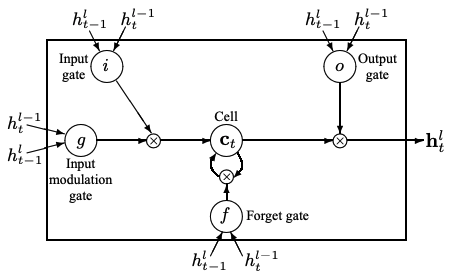
\includegraphics[width=0.5\textwidth]{figures/lstm.png}
  \caption{Graphical depiction of LSTM memory cells, from \cite{zaremba2014recurrent}}
  \label{fig:lstm}
\end{figure}

Per \cite{zaremba2014recurrent}, we initialized our first hidden state with zeros, and from there initialized the subsequent hidden states within a batch with the output of the last batch. Our LSTMs had 650 units per layer, and we additionally initialized LSTM parameters uniformly, with a weight bound of [-0.05, 0.05], applied a dropout rate of 0.5, and clipped gradients to a norm of 5 to prevent vanishing gradient problems.


\subsection{Calculating Perplexity}

Additionally, in this homework we were tasked with coming up with numerically stable ways to compute perplexity. Computers often have trouble computing very small sequence probabilities, so to avoid underflow problems, we used a derivation of perplexity that amounts to the exponentiated mean negative log likelihood of the probabilities of each constituent token:
\begin{align*}
  PP(x_{1:T}) &= [p(x_{1:T})]^{-\frac{1}{T}} \\
  &= [\prod_{i} p(x_i)] ^{-\frac{1}{T}} \\
  &= \prod_{i} [p(x_i) ^{-\frac{1}{T}}] \\
  &= \prod_{i} \exp\log(p(x_i) ^{-\frac{1}{T}}) \\
  &= \prod_{i} \exp[-\frac{1}{T}  \log(p(x_i))]\\
  &= \exp[ \sum_{i}(
    -\frac{\log(p(x_i))}{T} 
  ) ]\\
  PP(x_{1:T}) &= \exp[
    -\frac{\sum_{i}{\log(p(x_i))}}{T} 
  ]\\
\end{align*}

\section{Experiments}

The results of our experiments are depicted in Table \ref{tab:perplexities}. We now discuss results from each model.

\begin{table}[h]
  \centering
  \begin{tabular}{@{}lrrr@{}}
  \toprule
  \textbf{Model} & \textbf{PP(train)} & \textbf{PP(val)} & \textbf{PP(test)} \\ \midrule
  Trigram w/ Linear Interpolation & 12.6 & 45.2 & 46.7 \\
  Neural Network (random embedding initialization) & 397.2 & 415.0 & 388.5 \\ 
  Neural Network (pretrained embedding initialization) & 358.9 & 351.6 & 328.5 \\ 
  LSTM (random embedding initialization) & 138.5 & 150.0 & 139.5 \\ 
  LSTM (pretrained embedding initialization) & 87.3 & 119.0 & 111.0 \\ 
  \bottomrule
  \end{tabular}
  \caption{Perplexities of the implemented language models. Trigram model run with $a_1=0.7$, $a_2=0.2$. Neural network models trained for 10 epochs, $embed\_dim=300$, $lr=1e^{-3}$, $hidden\_dim=1200$. LSTM models trained for 5 epochs, $embed\_dim=300$, $lr=1e^{-5}$, $hidden\_dim=650$, $weight\_bound=0.05$, $dropout=0.5$.}
  \label{tab:perplexities}
\end{table}

\subsection{Trigram LM}

Our experiments with $a_1$ and $a_2$ are depicted in Table \ref{tab:a-pps}. As observed, the addition of bigram and trigram probabilities significantly lowered perplexity on training, validation and testing sets. 

Of note, these models handled out-of-vocabulary n-grams by first backing off to combinations of words with the unk token, which was abundant in the training corpus. If backing off to an unknown token still produces an unseen combination (e.g. \textit{(unk, unk, banana)} when the model has never seen `\textit{banana}' come after \textit{(unk, unk)}), the model assigns zero probability to the entire n-gram. Since the presence of the unknown token as a unigram in the training set meant unigram probabilities never backed off to 0, the perplexity values for the unigram-heavy interpolations appear inflated relative to those that gave higher weight to bigram and trigram probabilities. Further work should investigate other methods of out-of-vocabulary handling.

\begin{table}[h]
  \centering
  \begin{tabular}{@{}rrrrr@{}}
  \toprule
  \textbf{$a_1$} & \textbf{$a_2$} & \textbf{PP(train)} & \textbf{PP(val)} & \textbf{PP(test)} \\ \midrule
  0 & 0 & 684.9 & 687.0 & 639.2 \\
  0 & 0.50 & 115.5 & 103.0 & 103.9 \\
  0.33 & 0.33 & 19.7 & 47.3 & 48.5 \\
  0.70 & 0.20 & 12.6 & 45.2 & 46.7 \\
  0.10 & 0.20 & 44.0 & 77.9 & 79.2 \\
  \bottomrule
  \end{tabular}
  \caption{Effect of different $a$ on perplexity.}
  \label{tab:a-pps}
\end{table}

\subsection{Neural Network LM}

We experimented with two variations on the neural network specified in \cite{bengio2003neural}: one with randomly initialized embeddings $C$, and one initialized with pretrained embeddings pulled from the WikiVec corpus provided in the last assignment. As depicted in Figure \ref{fig:nn-pps}, both models were able to stabilize perplexities from high values close to initialization to more reasonable values within 5 epochs.

\begin{figure}[h]
  \centering
  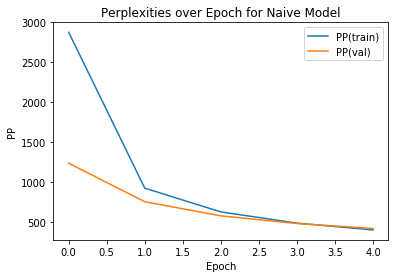
\includegraphics[width=0.45\textwidth]{figures/nn_naive_pp.png}
  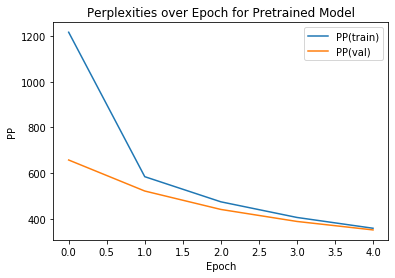
\includegraphics[width=0.45\textwidth]{figures/nn_pretrained_pp.png}
  \caption{Train- and val-set perplexities over epochs for neural network trigram models with (L) random embedding initialization and (R) pretrained embedding initialization. Within the first epoch the model begins to overfit to the training set. $lr=1e^{-3}$, $embed\_dim=300$}
  \label{fig:nn-pps}
\end{figure}

\subsection{LSTM}

Similarly, our LSTM results using random vs. pretrained embedding initialations show perplexities over epochs decrease steadily on both the training and validation sets (Figure \ref{fig:lstm-pps}). Notably, the pretrained LSTM in the run depicted was able to achieve a training perplexity below 100 (87.3, reported in Table \ref{tab:perplexities}) on the fifth epoch.

\begin{figure}
  \centering
  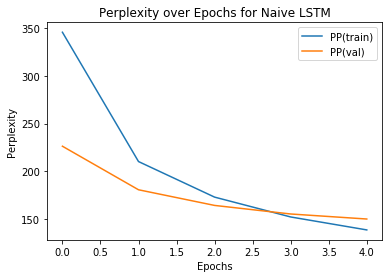
\includegraphics[width=0.45\textwidth]{figures/lstm_naive_pp.png}
  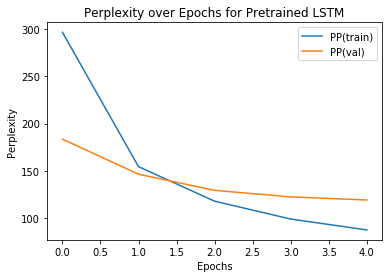
\includegraphics[width=0.45\textwidth]{figures/lstm_pretrained_pp.png}
  \caption{Train- and val-set perplexities over epochs for LSTM models with (L) random embedding initialization and (R) pretrained embedding initialization. $embed\_dim=300$, $lr=1e^{-3}$, $hidden\_dim=650$, $weight\_bound=0.05$, $dropout=0.5$}
  \label{fig:lstm-pps}
\end{figure}

\subsection{Extension 1}

We now report information theoretic analyses of each of the models for the following training and testing contexts: training batch 1 (1), training batch 7 (2), testing batch 117 (3), and testing batch 231 (4). The entropies of each context as assessed by each model are reported in Table \ref{tab:entropies}.
% \begin{enumerate}
%   \item ``\textit{president and chief executive officer of this financially troubled department store chain effective nov. N succeeding frank robertson who is retiring early $<$eos$>$ mr. $<$unk$>$ was previously president and chief operating officer}'' (training batch 1)
%   \item ``\textit{acceptance corp. N N N to N days N N N to N days N N N to N days N N N to N days N N N to N days}'' (training batch 7)
%   \item ``\textit{in london each giving buyers the right to buy one hong kong telecommunications share at a price to be determined friday $<$eos$>$ the N million warrants will be priced at hk\$ N}'' (testing batch 117)
%   \item ``\textit{john $<$unk$>$ $<$unk$>$ 's chief executive officer $<$eos$>$ at usa today ad pages totaled N for the quarter down N N from the N period which was helped by increased ad spending}'' (testing batch 231)
% \end{enumerate}

\begin{table}[h]
  \centering
  \begin{tabular}{@{}lrrrr@{}}
  \toprule
  \textbf{Model p} & \textbf{H(1$\sim$p)} & \textbf{H(2$\sim$p)} & \textbf{H(3$\sim$p)} & \textbf{H(4$\sim$p)} \\ \midrule
  Trigram w/ Linear Interpolation ($a_1=0.7$,$a_2=0.1$) & 2.5 & 2.5 & 4.0 & 3.9 \\
  Neural Network (pretrained embedding initialization) & 6.1 & 5.7 & 5.7 & 5.5 \\
  LSTM (pretrained embedding initialization) & 4.4 & 4.1 & 4.6 & 4.5 \\
  \bottomrule
  \end{tabular}
  \caption{Entropies of each training or testing context (above) under each model.}
  \label{tab:entropies}
\end{table}

\section{Conclusion}

In this assignment, we implemented several approaches to language modeling: (1) a count-based trigram model with linear interpolation; (2) variants on a neural network model; and (3) variants on an LSTM. Trained with and evaluated against data from the Penn Treebank \citep{marcus-etal-1993-building}. The resulting perplexity values (Tables \ref{tab:perplexities}, \ref{tab:a-pps}) show the LSTM models ``learned'' more rapidly than the neural networks, reaching lower perplexities in the same training timeframe (5 epochs). Further work might investigate approaches to fine-tuning the hyperparameters of these models for coherent comparisons of model efficacy, for example grid searches for efficient learning rates.

This assignment also highlighted practical considerations for implementing perplexity calculations. While conceptually straightforward, in practice it is clear further debugging is needed to work out why the perplexity values vary so greatly within the trigram models.

Finally, at submission time neither extension had been completed. We look to these as future areas of work.

\bibliographystyle{apalike}
\bibliography{hw2-writeup}

\end{document}
